\documentclass[11pt,a4paper]{article}

\usepackage[utf8]{inputenc}
\usepackage[T1]{fontenc}
\usepackage{lmodern}
\usepackage[spanish,es-tabla]{babel}
\usepackage[margin=2.5cm]{geometry}
\usepackage{amsmath,amssymb}
\usepackage{graphicx}
\usepackage{booktabs}
\usepackage{xcolor}
\usepackage[hidelinks]{hyperref}

% Las figuras se leen directamente de results/
\graphicspath{{../results/}}

% Marca de texto pendiente.
\newcommand{\pendiente}[1]{\textcolor{red}{[PENDIENTE: #1]}}

\title{Consistency Models}
\author{Ibon De Mingo Arroyo \and Eloísa Denia García \and Matin Esmaeilzadeh}
\date{Noviembre de 2026}

\begin{document}

\maketitle

\begin{abstract}
\pendiente{}
\end{abstract}

% ---------------------------------------------------------------------------
\section{Introducción}
\label{sec:introduccion}

Los modelos de difusión~\cite{ho2020ddpm,song2021sde} son hoy una de las
familias de modelos generativos de imágenes con mejores resultados. Su idea
consiste en destruir los datos poco a poco añadiéndoles ruido y entrenar una
red neuronal que aprenda a invertir ese proceso. El precio de esta calidad es
el coste de generación: para obtener una sola imagen hay que partir de ruido
puro y eliminarlo paso a paso, evaluando la red en cada uno de ellos. Ho et
al.~\cite{ho2020ddpm} utilizan 1000 pasos por muestra. Formular el proceso
como una ecuación diferencial ordinaria, la \emph{probability flow
ODE}~\cite{song2021sde}, permite reducir mucho esa cifra, pero sigue siendo
necesario evaluar la red decenas de veces por imagen.

Para resolver este problema, Song et al.~\cite{song2023consistency}
propusieron los \emph{Consistency Models}. Un modelo de consistencia aprende a
llevar cualquier punto de una trayectoria de esa ecuación directamente a su
origen, es decir, a la imagen limpia en la que termina la trayectoria. Gracias
a ello puede generar una muestra con una sola evaluación de la red. Si se
dispone de más presupuesto de cómputo, puede además encadenar varios pasos,
volviendo a añadir ruido y eliminándolo de nuevo, para mejorar la calidad. El
artículo presenta dos formas de entrenarlos: \emph{consistency distillation}
(CD), que destila el conocimiento de un modelo de difusión ya entrenado que
actúa como maestro, y \emph{consistency training} (CT), que los entrena desde
cero, sin maestro.

El objetivo de este proyecto es reproducir esta metodología a pequeña escala
sobre MNIST~\cite{lecun1998mnist} y medir qué se gana y qué se pierde al
reducir el número de pasos de generación. Se ha elegido MNIST porque es un
conjunto de datos ligero, que permite entrenar varios modelos completos dentro
del plazo del proyecto y sin GPU.

Respecto a la propuesta inicial, el proyecto se ha ampliado en una dirección:
además del maestro de difusión, se ha entrenado un segundo maestro basado en
Rectified Flow~\cite{liu2023flow}, y también se ha destilado en un modelo de
consistencia. Esto permite estudiar cómo influye el tipo de maestro en el
modelo resultante.

\subsection{Objetivos}

Los objetivos principales planteados en la propuesta del proyecto son:
\begin{enumerate}
  \item Entrenar un modelo de difusión que sirva como maestro para el modelo
        de consistencia.
  \item Destilar el conocimiento aprendido por el modelo maestro en un modelo
        de consistencia más rápido.
  \item Comparar el modelo de consistencia frente al modelo de difusión en
        términos de velocidad y calidad de generación.
  \item Estudiar los resultados: la aceleración obtenida, la calidad de las
        imágenes generadas con más o menos pasos y su diversidad, además de
        otras cuestiones técnicas de interés y las limitaciones encontradas.
\end{enumerate}
Una vez cumplidos estos objetivos, la propuesta contemplaba tres extensiones,
en este orden: entrenar el modelo mediante consistency training y compararlo
con los anteriores; adaptar la arquitectura a imágenes en color con
CIFAR-10~\cite{krizhevsky2009cifar}; y desarrollar un modelo de consistencia
condicional, capaz de generar un dígito concreto.

Los cuatro objetivos principales se han cumplido.
\pendiente{decidir qué extensiones se incluyen en la entrega}

\subsection{Estructura del documento}

La sección~\ref{sec:metodologia} describe los modelos implementados (los dos
maestros, la destilación a modelos de consistencia y su muestreo), las
diferencias respecto al artículo original y cómo se han evaluado los modelos.
La sección~\ref{sec:resultados} presenta los resultados obtenidos. Por último, la
sección~\ref{sec:discusion} los analiza junto con las limitaciones del
trabajo, y la sección~\ref{sec:conclusiones} recoge las conclusiones.

% ---------------------------------------------------------------------------
\section{Metodología}
\label{sec:metodologia}
\pendiente{escribir cuando los modelos sean definitivos. Hay un borrador en
\texttt{borrador\_metodologia.tex}.}

\subsection{Datos y arquitectura}
\pendiente{MNIST y la U-Net común a todos los modelos.}

\subsection{Modelos maestros}
\pendiente{maestro de difusión VE, maestro Rectified Flow y reflow.}

\subsection{Modelos de consistencia}
\pendiente{parametrización, consistency distillation de CM-VE y CM-RF, y
consistency training.}

\subsection{Muestreo de los modelos de consistencia}
\pendiente{generación en uno y en varios pasos.}

\subsection{Diferencias respecto al artículo original}
\pendiente{diferencias de la reproducción respecto a Song et al.}

\subsection{Protocolo de evaluación}
\label{sec:evaluacion}
% Parte cerrada: no depende de los checkpoints finales.

\paragraph{Clasificador de referencia}
\pendiente{CNN, 421\,642 pesos, 99{,}00\,\% en test, 10 épocas.}

\paragraph{Métricas de calidad y diversidad}
\pendiente{FD-MNIST (distancia de Fréchet sobre las 128 features del clasificador,
como FID \cite{heusel2017fid}); porcentaje de muestras reconocibles
(confianza $>0{,}9$); entropía de la distribución de dígitos.
Explicar por qué FD es la métrica principal: el clasificador marca el 61\,\%
del ruido puro como dígito con confianza alta. Referencias: MNIST real y ruido puro.}

\paragraph{Medida de tiempos}
\pendiente{ms por imagen, NFE, tiempo frente a $N$, hardware (CPU), $N_\text{eval}=2000$.}

% ---------------------------------------------------------------------------
\section{Resultados}
\label{sec:resultados}
% Depende de los checkpoints finales. Redactar con los números actuales
% y revisar cuando se vuelva a ejecutar compare.py.

\pendiente{todas las figuras y números de esta sección son provisionales.
Eloísa está reentrenando CM-RF y los resultados actuales de CM-RF están
evaluados de forma incorrecta (con $c_\text{in}$, aunque se entrenó sin él).
Cuando estén los checkpoints finales, actualizar \texttt{MODELS} en
\texttt{compare.py}, volver a ejecutarlo y revisar el texto, la tabla y las
figuras (las figuras se actualizan solas al recompilar).}

\subsection{Calidad frente al número de pasos}
\pendiente{tabla de resultados y comentario.}

\begin{figure}[ht]
  \centering
  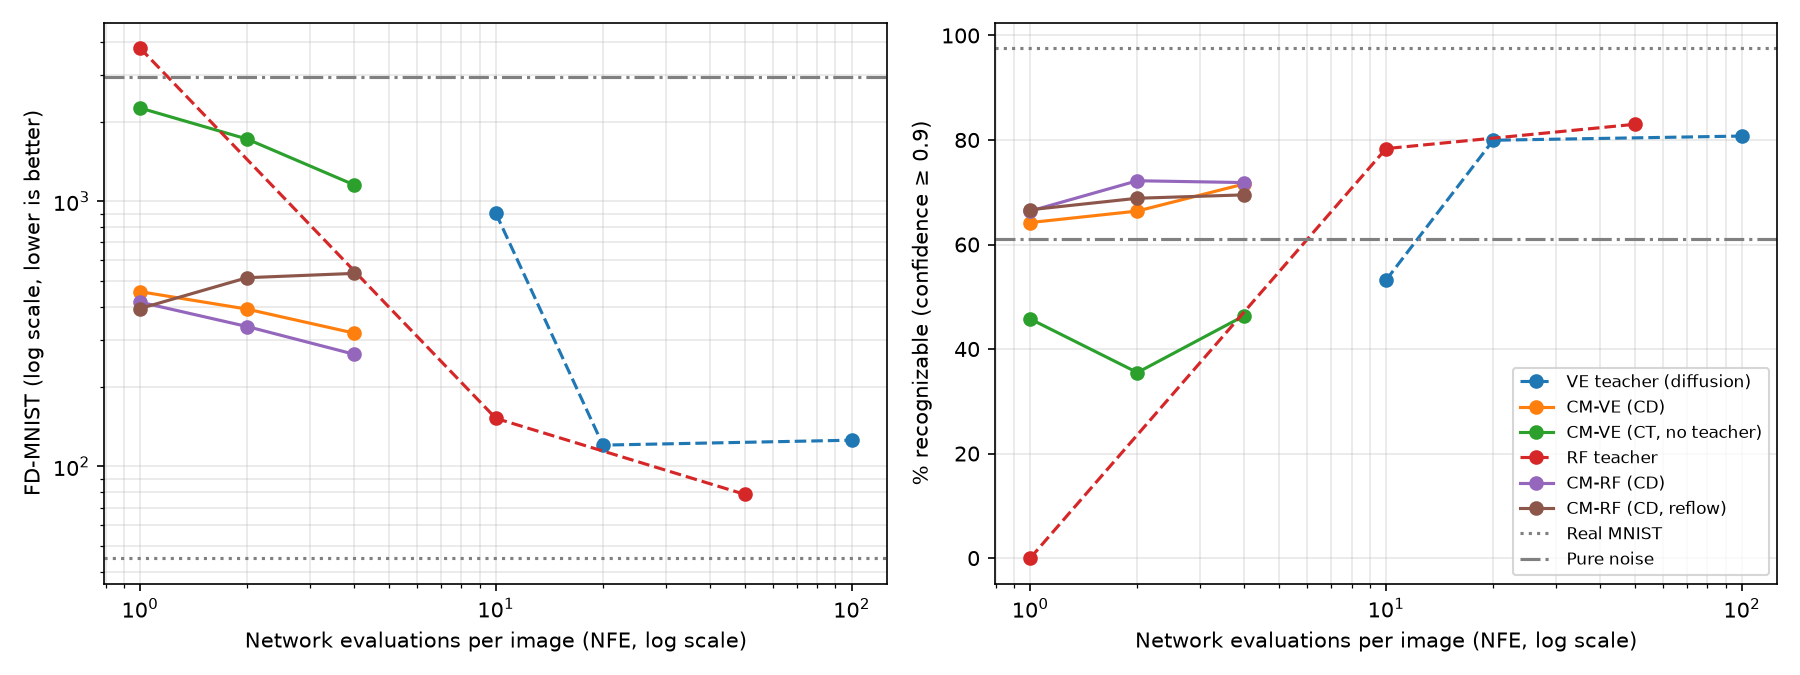
\includegraphics[width=0.8\linewidth]{calidad_vs_nfe.png}
  \caption{FD-MNIST frente al número de evaluaciones de la red (NFE).}
  \label{fig:calidad_nfe}
\end{figure}

\subsection{Velocidad de generación}
\begin{figure}[ht]
  \centering
  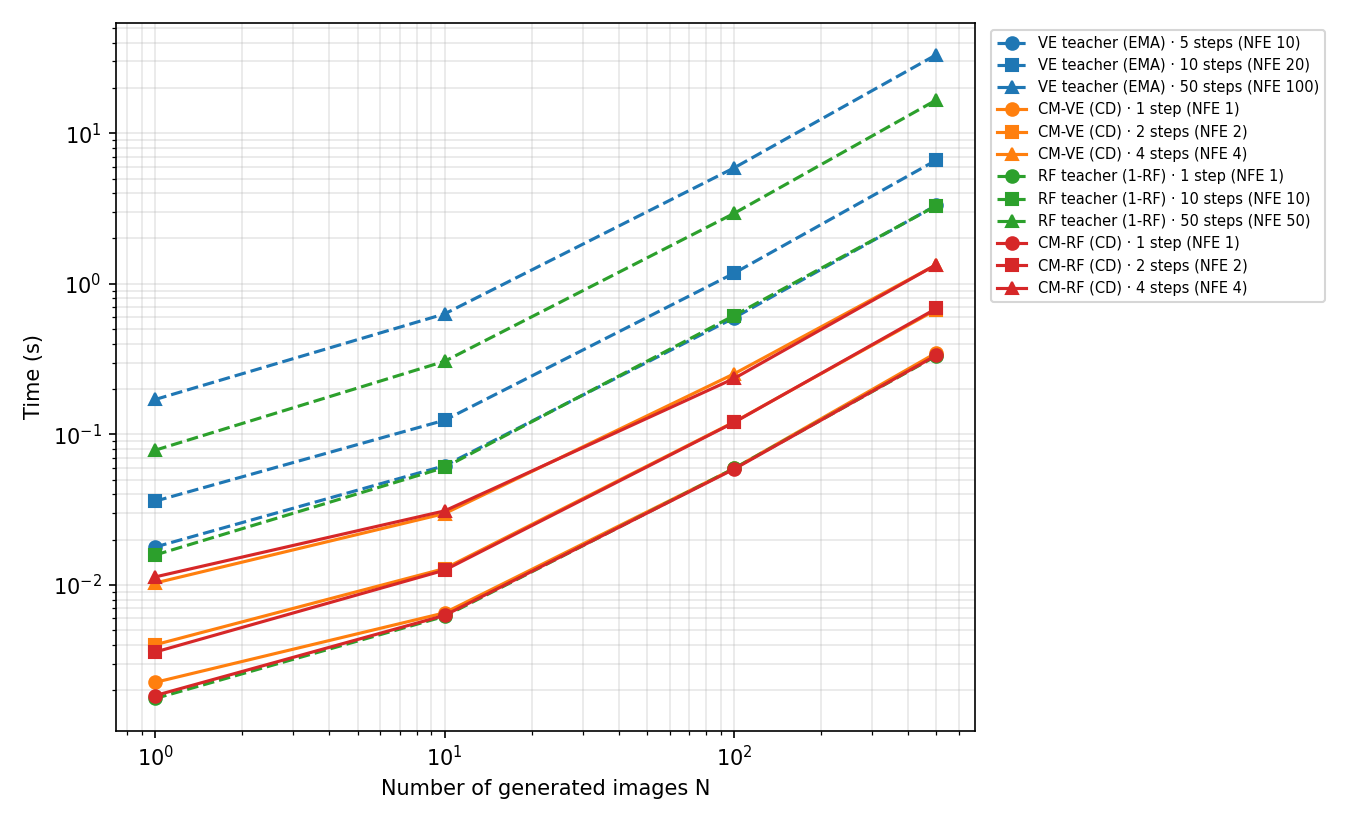
\includegraphics[width=0.8\linewidth]{tiempo_vs_n.png}
  \caption{Tiempo de generación frente al número de muestras $N$.}
  \label{fig:tiempo_n}
\end{figure}
\pendiente{aceleración frente al maestro con 50 y con 10 pasos.}

\subsection{Diversidad}
\begin{figure}[ht]
  \centering
  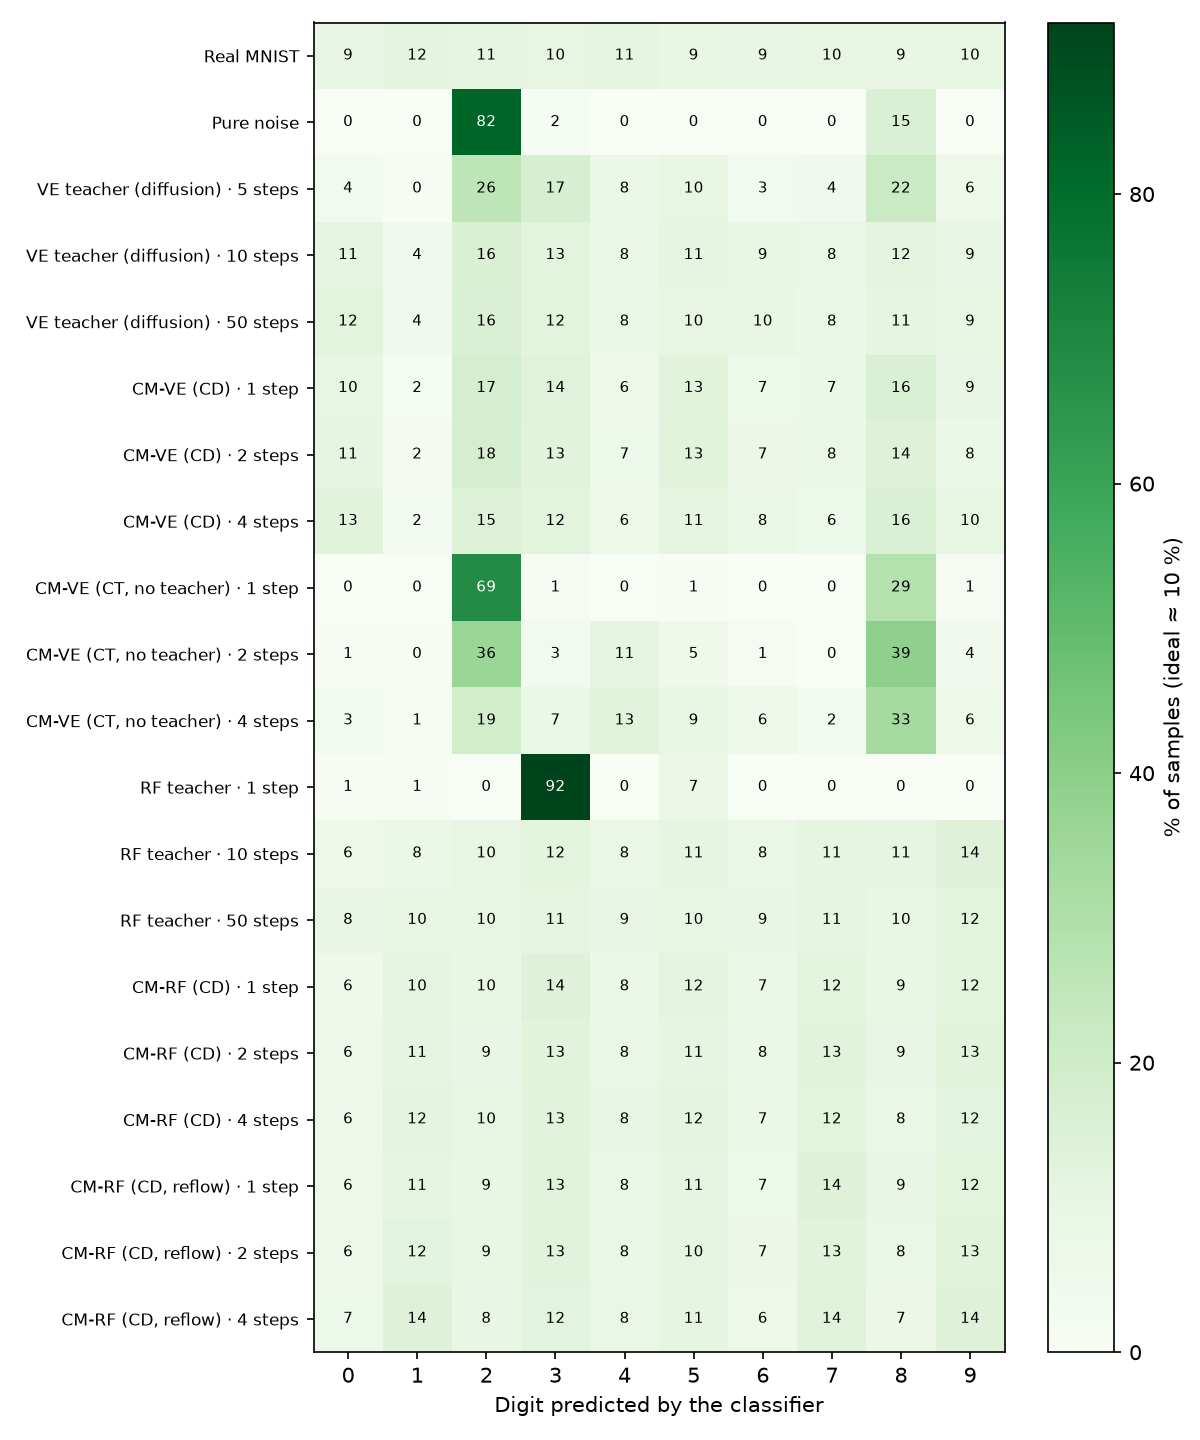
\includegraphics[width=0.9\linewidth]{distribucion_digitos.png}
  \caption{Distribución de dígitos predichos por el clasificador.}
  \label{fig:distribucion}
\end{figure}
\pendiente{entropía, sesgo heredado del maestro (pocos ``1''), colapso de CT.}

\subsection{Inspección visual}
\begin{figure}[ht]
  \centering
  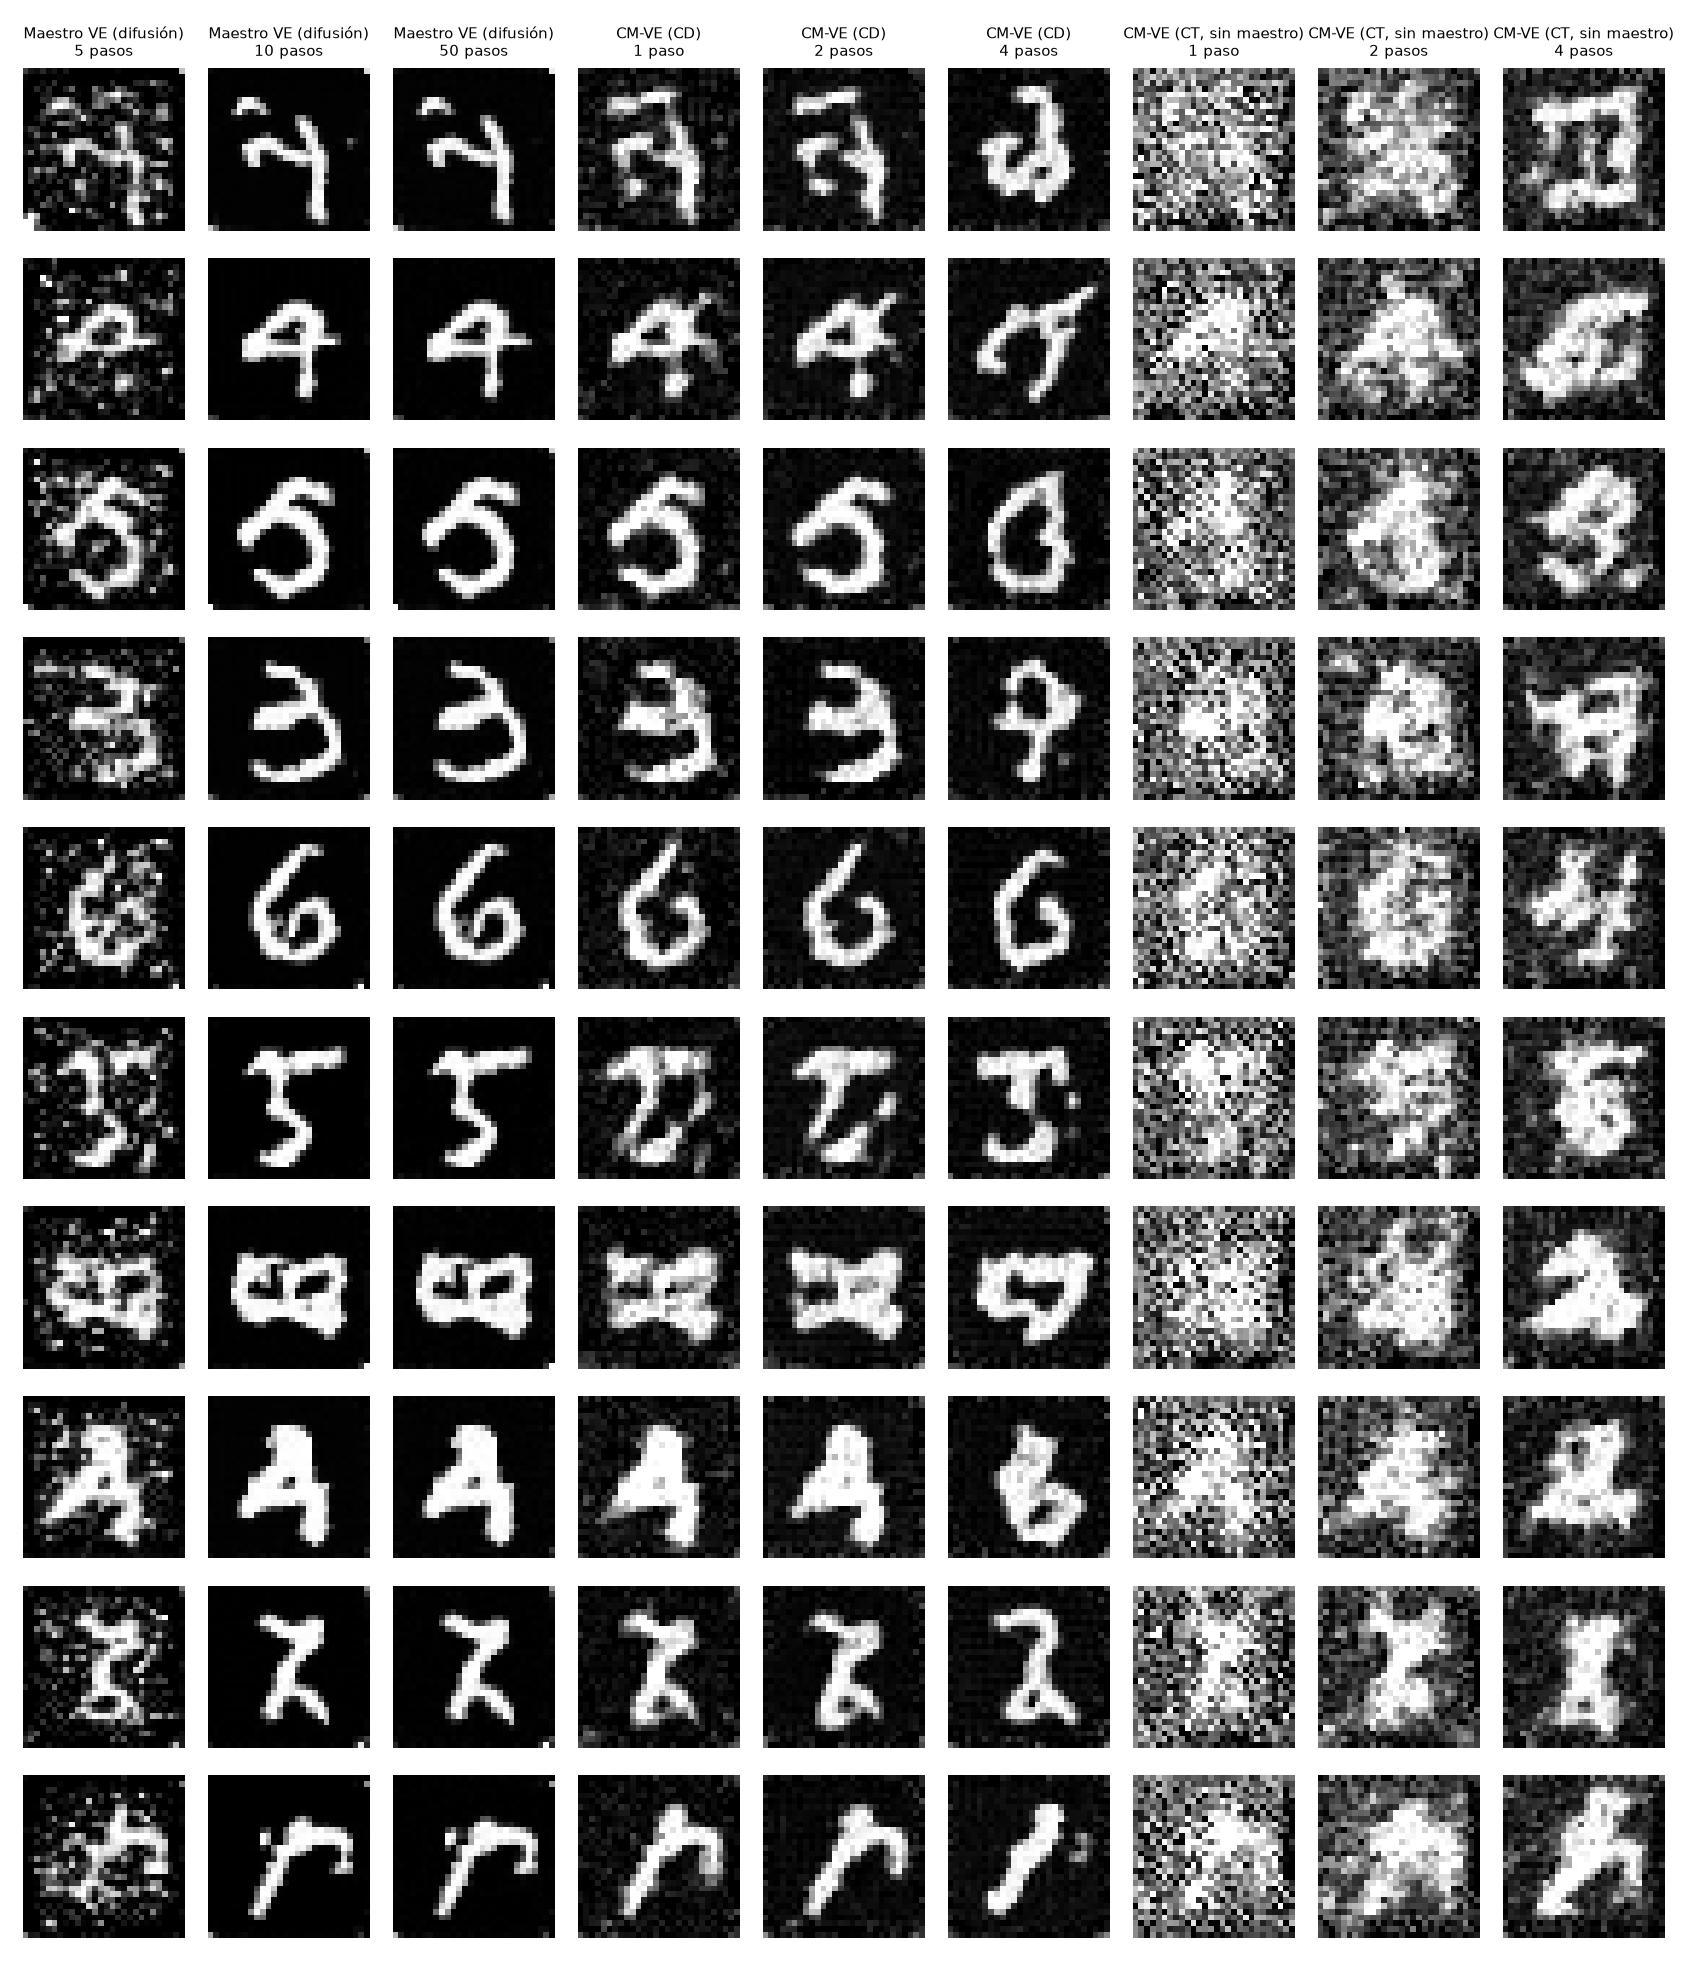
\includegraphics[width=0.48\linewidth]{muestras_ve.png}\hfill
  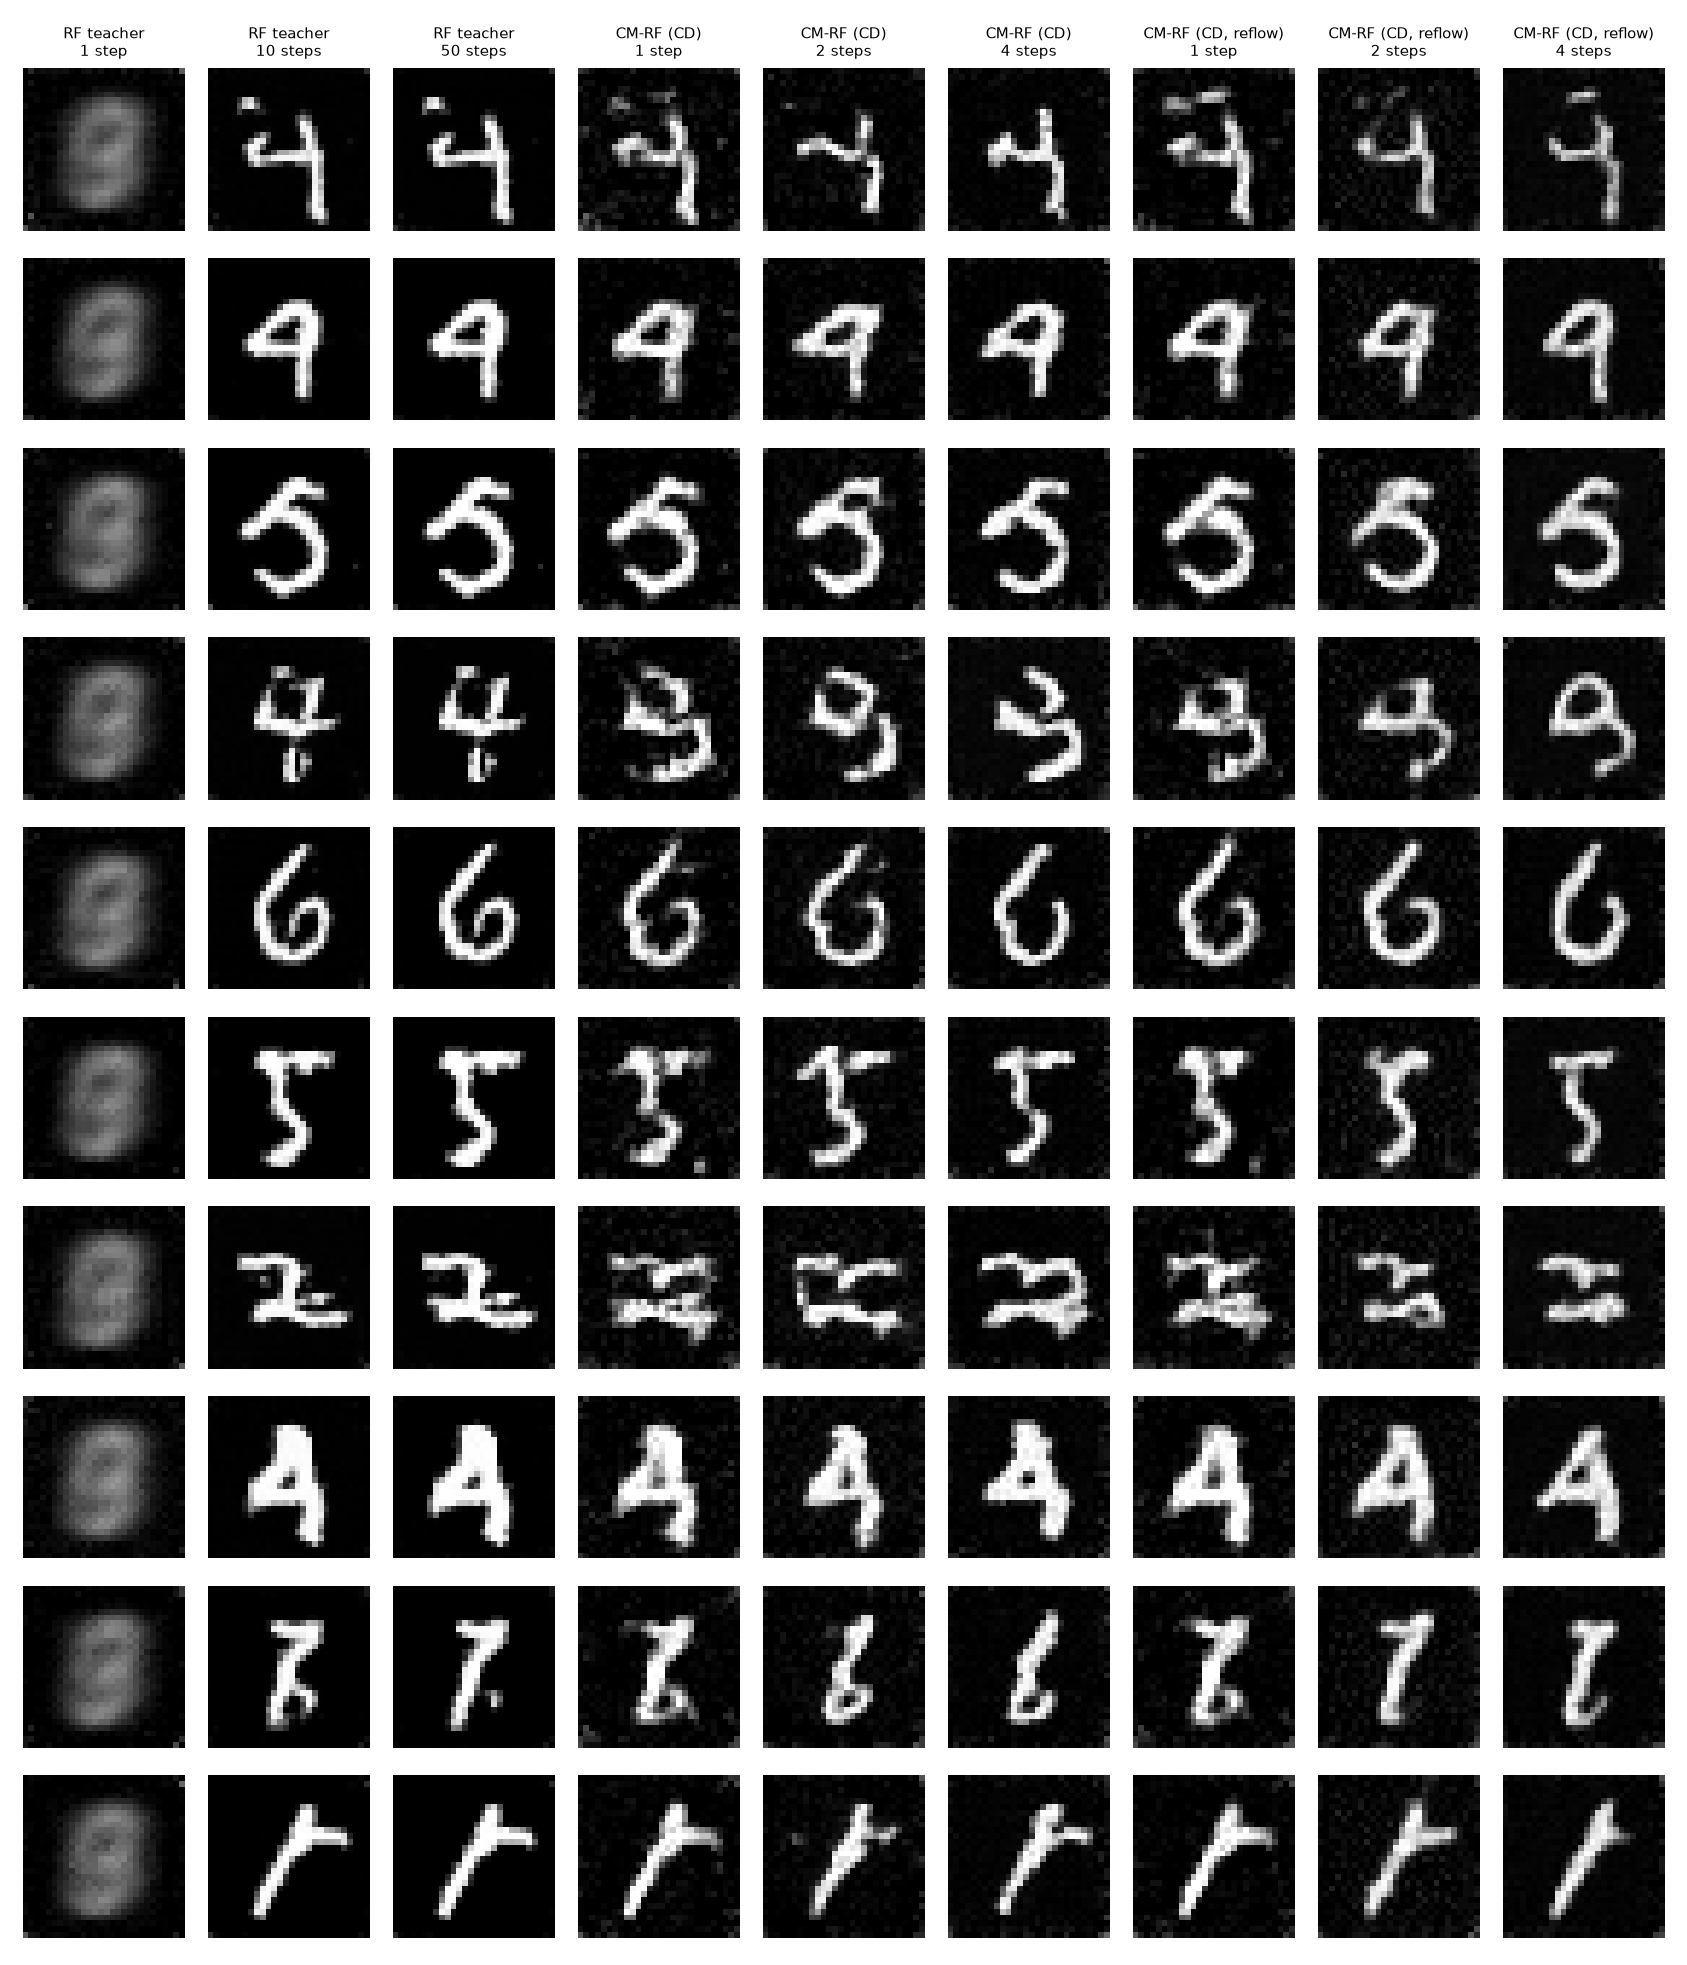
\includegraphics[width=0.48\linewidth]{muestras_rf.png}
  \caption{Muestras de la familia VE (izquierda) y RF (derecha).}
  \label{fig:muestras}
\end{figure}

% ---------------------------------------------------------------------------
\section{Discusión y limitaciones}
\label{sec:discusion}
\pendiente{qué se gana y qué se pierde al reducir pasos; VE frente a RF como
maestro; por qué CT y reflow no funcionan; limitaciones (CPU, tamaño de red,
métrica basada en un clasificador propio). Escribir solo con los resultados
finales: la comparación VE frente a RF depende del reentrenamiento de CM-RF.}

% ---------------------------------------------------------------------------
\section{Conclusiones y trabajo futuro}
\label{sec:conclusiones}
\pendiente{cumplimiento de objetivos; extensiones no realizadas (CIFAR-10 \cite{krizhevsky2009cifar},
modelo condicional) y por qué.}

\bibliographystyle{unsrt}
\bibliography{referencias}

\end{document}
